\documentclass[a4paper]{article}
\usepackage[margin=1in]{geometry}
\usepackage[english]{babel}
\usepackage[utf8]{inputenc}
\usepackage{amsmath}
\usepackage{graphicx}
\usepackage{amssymb}
\usepackage{amsthm}
\usepackage{tikz-cd}
\usepackage{mathrsfs}
\usepackage[colorinlistoftodos]{todonotes}
\usepackage{enumitem}
\usepackage{yfonts}
\usepackage{dsfont}
\usepackage{mathtools}
\usepackage{hyperref}
\DeclarePairedDelimiter\ceil{\lceil}{\rceil}
\DeclarePairedDelimiter\floor{\lfloor}{\rfloor}

\title{Randomized Algorithms Notes}
\author{Wilson Pan}
\date{\today}

\newtheorem{thm}{Theorem}[section]
\newtheorem{lem}[thm]{Lemma}
\newtheorem{defn}[thm]{Definition}
\newtheorem{eg}[thm]{Example}
\newtheorem{ex}[thm]{Exercise}
\newtheorem{conj}[thm]{Conjecture}
\newtheorem{cor}[thm]{Corollary}
\newtheorem{claim}[thm]{Claim}
\newtheorem{rmk}[thm]{Remark}

\newcommand{\ie}{\emph{i.e.} }
\newcommand{\cf}{\emph{cf.} }
\newcommand{\into}{\hookrightarrow}
\newcommand{\dirac}{\slashed{\partial}}
\newcommand{\R}{\mathbb{R}}
\newcommand{\C}{\mathbb{C}}
\newcommand{\Z}{\mathbb{Z}}
\newcommand{\N}{\mathbb{N}}
\newcommand{\Q}{\mathbb{Q}}
\newcommand{\LieT}{\mathfrak{t}}
\newcommand{\T}{\mathbb{T}}
\newcommand{\A}{\mathds{A}}
\newcommand{\HG}{\mathcal{H}}
\newcommand{\F}{\mathbb{F}}
\newcommand{\poly}[2]{\text{Poly}_{#1}(#2)}
\newcommand{\gen}[1]{\langle #1 \rangle}
\newcommand{\Hom}{\text{Hom}}
\newcommand{\E}{\mathbb{E}}

\usepackage{tikz}
\usetikzlibrary{arrows.meta, positioning, calc, shapes.geometric}
\begin{document}
\maketitle
\tableofcontents
\newpage
\section{Jan 4}
\subsection{Background}

Before analyzing the main problem, we briefly review two important concepts that will be central to our solution: the cycle decomposition of permutations and Markov's Inequality.

\subsubsection{Permutations and Cycle Notation}
A permutation $\sigma$ of the set $\{1, \dots, n\}$ is a bijection from the set to itself. We can decompose any permutation into disjoint cycles.
\begin{eg}
    Consider the permutation defined by:
    \[
    \sigma = \begin{pmatrix} 
        1 & 2 & 3 & 4 & 5 & 6 & 7 & 8 & 9 & 10 \\ 
        7 & 6 & 4 & 3 & 8 & 1 & 2 & 9 & 5 & 10 
    \end{pmatrix}
    \]
    In disjoint cycle notation, this is written as $(1\; 7\; 2\; 6)(3\; 4)(5\; 8\; 9)(10)$. We can visualize this decomposition below:
    
    \begin{center}
    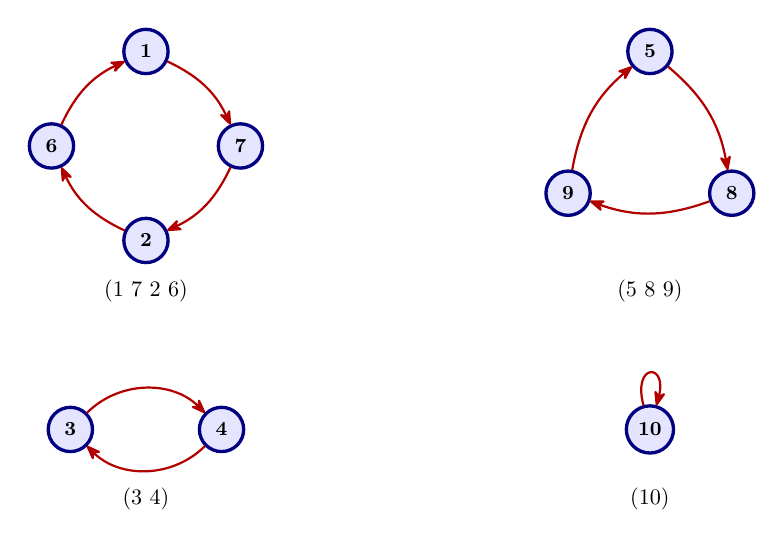
\begin{tikzpicture}[
        vertex/.style={
            circle,
            draw=blue!50!black,
            fill=blue!10,
            very thick,
            minimum size=20pt,
            font=\small\bfseries
        },
        edge/.style={
            ->,
            >={Stealth[round]}, 
            draw=red!70!black,
            thick,
            bend left=20
        },
        selfloop/.style={
            ->,
            >={Stealth[round]},
            draw=red!70!black,
            thick,
            loop above,
            min distance=20pt
        },
        scale=0.8, transform shape
    ]

    \coordinate (C1) at (-4, 2);  
    \coordinate (C2) at (4, 2);   
    \coordinate (C3) at (-4, -2.5); 
    \coordinate (C4) at (4, -2.5);  

    \node[vertex] (n1) at ($(C1) + (90:1.5cm)$) {1};
    \node[vertex] (n7) at ($(C1) + (0:1.5cm)$)  {7};
    \node[vertex] (n2) at ($(C1) + (270:1.5cm)$){2};
    \node[vertex] (n6) at ($(C1) + (180:1.5cm)$){6};

    \draw[edge] (n1) to (n7);
    \draw[edge] (n7) to (n2);
    \draw[edge] (n2) to (n6);
    \draw[edge] (n6) to (n1);
    \node[below=2cm of C1] {(1 7 2 6)};

    \node[vertex] (n5) at ($(C2) + (90:1.5cm)$)  {5};
    \node[vertex] (n8) at ($(C2) + (330:1.5cm)$) {8};
    \node[vertex] (n9) at ($(C2) + (210:1.5cm)$) {9};

    \draw[edge] (n5) to (n8);
    \draw[edge] (n8) to (n9);
    \draw[edge] (n9) to (n5);
    \node[below=2cm of C2] {(5 8 9)};

    \node[vertex] (n3) at ($(C3) + (-1.2, 0)$) {3};
    \node[vertex] (n4) at ($(C3) + (1.2, 0)$)  {4};

    \draw[edge, bend left=45] (n3) to (n4);
    \draw[edge, bend left=45] (n4) to (n3);
    \node[below=0.8cm of C3] {(3 4)};

    \node[vertex] (n10) at (C4) {10};
    \draw[selfloop] (n10) to (n10);
    \node[below=0.8cm of C4] {(10)};

    \end{tikzpicture}
    \end{center}
\end{eg}

\subsubsection{Probabilistic Tools}
We will also make use of Markov's Inequality to bound probabilities.

\begin{thm}[Markov's Inequality]
    If $X$ is a non-negative random variable and $k > 0$ then:
    \[
    \mathbb{P}[X\geq k\cdot \mathbb{E}[X]]\leq \frac{1}{k}.
    \] 
\end{thm}
\subsection{100 Prisoners Problem:} In a prison, there are $100$ prisoners and there is a warden who want to retire. He decides to play a game.
    \begin{enumerate}
        \item In a room there are $100$ boxes, In these boxes, is a permutation of the numbers $1,2,...,100$. The boxes are closed and the prisoners cannot see the numbers within the boxes.
        \item The prisoners will each enter and play a mini-game. For the $i$-th prisoner, they open $50$ boxes and wins by finding the number $i$.
        \item After a prisoner leaves, the boxes are closed again, and the state of the room is restored to exactly how it was before they entered. Prisoners cannot communicate after the game begins.
        \item Prisoners win the game (and survive) if and only if \textbf{every} prisoner finds their own number. Otherwise, they are all executed.
    \end{enumerate}
\noindent \textbf{Naive Algorithm:} Each prisoner opens $50$ random boxes then \[
\mathbb{P}[\text{Victory}] = \left(\frac{1}{2}\right)^{100} \approx 8 \times 10^{-31}.
\]
\subsection{Cycle Following Algorithm}

We propose a strategy that utilizes the permutation structure inside the boxes.\\
\textbf{Cycle Algorithm:} 
    Consider the algorithm where person $i$ opens box $i$, sees $j$, then open box $j$, see $k$ and so on. This continues until they find their number or exhaust their $50$ tries.

\begin{lem}
    Under the Cycle Algorithm, prisoner $i$ succeeds if and only if $i$ belongs to a cycle of length less than or equal to 50. Consequently, the team achieves victory if and only if the permutation contains no cycle of length strictly greater than 50.
\end{lem}
\subsubsection{A Warm-up Bound using Markov's Inequality}
Before calculating the exact probability, let us try to bound the failure probability of a slightly easier version of the game using Markov's Inequality.

\begin{lem}
    Consider a variant where each prisoner is allowed to open 75 boxes. Using the Cycle Algorithm, the probability of failure is at most $1/3$.
    \begin{proof}
        Let $X$ be the number of prisoners who lose. We write \[
        X = \sum_{i=1}^{100} I_i \text{ where } I_i=\begin{cases}
            1 & \text{if prisoner $i$ loses} \\
            0 & \text{otherwise} 
        \end{cases}
        .\]
        First, observe that for any prisoner $i$, the probability that their specific number lies in the 25 unopened boxes is exactly $25/100 = 1/4$. Thus, $\mathbb{E}[I_i] = 1/4$. By linearity of expectation:
        \[
        \mathbb{E}[X] = \sum_{i=1}^{100} \mathbb{E}[I_i] = 100 \cdot \frac{1}{4} = 25.
        \]\\
        Now, observe the Cycle Algorithm: If prisoner $i$ loses, they must be part of a cycle of length greater than 75. As cycles are disjoint, anyone else with a number in that same cycle will also lose. Therefore, if anyone loses like when $X>0$, then strictly more than 75 people must lose so $X>75$.\\
        Using Markov's Inequality with $k=3$:
        \[
        \mathbb{P}[\text{Non-victory}] = \mathbb{P}[X > 0] = \mathbb{P}[X \geq 76] \leq \mathbb{P}[X \geq 75] \leq \frac{\mathbb{E}[X]}{75} = \frac{25}{75} = \frac{1}{3}.
        \]
    \end{proof}
\end{lem}
\subsubsection{Exact Probability Calculation}

\begin{thm}
    The Cycle Algorithm achieves a victory probability of $\mathbb{P}[\text{Victory}] \approx 0.31$.
    \begin{proof}
        The prisoners fail if and only if there exists a cycle of length $\ell > 50$. Since the sum of cycle lengths is 100, there can be at most one cycle of length greater than 50. Thus, the events of having a cycle of length $\ell$ (for $\ell > 50$) are mutually exclusive.
        \[
        \mathbb{P}[\text{Non-victory}] = \mathbb{P}[\exists \text{ cycle of length } > 50] = \sum_{\ell=51}^{100} \mathbb{P}[\exists \text{ cycle of length } \ell].
        \]
        To calculate the number of permutations of $N=100$ elements that contain a cycle of length exactly $\ell$.
        \begin{enumerate}
            \item Choose $\ell$ elements to be in the cycle: $\binom{N}{\ell}$ ways
            \item Arrange these $\ell$ elements into a cycle: $(\ell-1)!$ ways
            \item Permute the remaining $N-\ell$ elements arbitrarily: $(N-\ell)!$ ways
        \end{enumerate}
        The total number of such permutations is:
        \[
        \binom{N}{\ell} \cdot (\ell - 1)! \cdot (N - \ell)! = \frac{N!}{\ell!(N-\ell)!} (\ell - 1)! (N - \ell)! = \frac{N!}{\ell}.
        \]
        The probability that a random permutation contains a cycle of length $\ell$ is therefore:
        \[
         \frac{N! / \ell}{N!} = \frac{1}{\ell}.
        \]
        Summing these probabilities:
        \[
         \mathbb{P}[\text{Non-victory}] = \sum_{\ell=51}^{100} \frac{1}{\ell} = H_{100} - H_{50} \approx \ln(100) - \ln(50) = \ln(2) \approx 0.69.
        \]
        Thus, the probability of victory is $1 - 0.69 \approx 0.31$.
    \end{proof}
\end{thm}
\begin{thm}
    The previous algorithm is optimal. 
    \begin{proof}
        Consider a second version of the game:
        \begin{enumerate}
            \item Prisoner 1 enters, opens 50 boxes 
            \item The difference between the games is that the boxes \textbf{remain open} for subsequent prisoners
            \item Prisoner $i$ enters. They win immediately if their box was already opened. Otherwise they may open more boxes until 50 total boxes (including those opened by previous prisoners) have been opened in the room
        \end{enumerate}
        We rely on the following two lemmas to complete the theorem.
    \end{proof}
\end{thm}
\begin{lem}
    The Cycle Algorithm achieves victory in Game 2 if and only if there are no cycles of length greater than 50.
    \begin{proof}
        Consider when there are no cycles of length $>50$, the Cycle Algorithm wins Game 1, and since Game 2 provides more information as boxes stay opened, it also wins Game 2.
        Conversely, suppose there is a cycle of length $>50$. The first prisoner in that cycle to enter the room will be forced to open the boxes in that cycle, since the boxes were closed before they entered or if open, did not contain their number, they must follow the cycle. They will run out of their 50 openings before finding their number. Thus, the team fails. Therefore, the performance of the Cycle Algorithm is identical in Game 1 and Game 2.
    \end{proof}
\end{lem}
\begin{lem}
    In Game 2, all strategies yield the same probability of victory.
    \begin{proof}
        In Game 2, the boxes remain open, this means the decision of which box to open next depends on the set of boxes currently revealed. However, since the permutation inside the boxes is chosen uniformly, the values hidden in the unopened boxes are a random permutation of the remaining numbers.\\ 
        Consequently, the probability that the \emph{next} box opened contains a specific required number depends only on the number of boxes remaining, not on which specific box is chosen. Regardless of the strategy used, the probability that the union of opened boxes contains the set of all prisoners' numbers is not changed.
    \end{proof}
\end{lem}
\noindent \textbf{Conclusion of Optimality:}
We have established the following chain of inequalities:
\[
\mathbb{P}(\text{Cycle wins Game 1}) \leq \mathbb{P}(\text{Optimal Strategy wins Game 1}) \leq \mathbb{P}(\text{Optimal Strategy wins Game 2}).
\]
The second inequality is true as any strategy for Game 1 is a strategy for Game 2 if we ignore the extra information, so Game 2 is strictly easier.
However, by Lemma 4.3, all strategies in Game 2 are equivalent.
\[
\mathbb{P}(\text{Optimal Strategy wins Game 2}) = \mathbb{P}(\text{Cycle wins Game 2}).
\]
And by Lemma 4.2:
\[
\mathbb{P}(\text{Cycle wins Game 2}) = \mathbb{P}(\text{Cycle wins Game 1}).
\]
Combining these we get:
\[
\mathbb{P}(\text{Cycle wins Game 1}) \leq \mathbb{P}(\text{Optimal Strategy wins Game 1}) \leq \mathbb{P}(\text{Cycle wins Game 1}).
\]
Therefore, the inequalities must be equalities, and the Cycle Algorithm is optimal for Game 1.
\newpage
\section{Jan 21}
\subsection{Mcdiarmid's Theorem}
\begin{thm}
    Mcdiarmid's Theorem (1993) Given 3-colorable graph, we can efficiently compute a triangle-free partition. \\
    The algorithm is in each round \begin{enumerate}
        \item Find some triangle in some part
        \item Pick random vertex in the triangle
        \item Move vertex to other side
    \end{enumerate}
    \begin{proof}
        Pick a specific $3$ coloring of the graph then let $X=$ \# color $1$ vertices on left and $Y=$ \# color $2$ vertices on right side. Observe that the value $X+Y$ changes by $ \{-1,0,1\}$ with equal probability. Then observe a random walk in $[0,n]$ \\
        \begin{lem}
            Let $T(n)=\E[ \text{time to get to }\pm n]$ then $T(n)=n^2$, but we restrict it to powers of $2$.\\
            We can easily see the following recurrence holds and it implies the lemma \[
            T(n)=T \left( \frac{n}{2} \right)+ T \left( \frac{n}{2} \right)+\frac{1}{2}T(n)
            .\] 
        \end{lem}
    \end{proof}
    So the expected number of rounds is $O \left( n^2 \right)$
\end{thm}
\subsection{Some theorem}
\begin{thm}
    Given $G=(V,E)$ we want for each pair $x,y\in V$ to calculate $d(x,y)\pm 2$. We will do it in $O(n^{2.5}\ln n)$.
\end{thm}
\begin{proof}
    Consider the shortest path $x\to y$ 
    \begin{enumerate}
        \item[Option 1:] Path has no vertices with degree $>\sqrt{n}$. We can run BFS from each node, but exclude high degree nodes from search. So $O(|V|\cdot n^{1.5})=O(n^{2.5})$
        \item[Option 2:] There exist a high degree vertex on $x\to y$ path. Define $S=100\sqrt{n}\log n$ vertices, each of which is an independent uniform random vertex. 
    \end{enumerate}
    Claim: With good probability, every high-degree vertex is incident to at least one vertex in $S$. \\
    Observe that there exist $s\in S$ such that \[
    d(x,s)+d(s,y)\leq d(x,y)+2
    .\]
    For each $s\in S$ do BFS and this runs at $O(n^{2.5} \log n)$
    Then for each $x,y$ compute \[
    \min_{s\in S}d(x,s)+d(s,y)
    .\] 
    This also is $O(n^{2.5}\log n).$
    \begin{align*}
        \Pr[ \text{given high degree vertex } w\not \sim S]&\leq \Pr[ \text{every sample misses neigh}(c_v)]\\
        &\leq \left(  1-\frac{1}{\sqrt{n}} \right)^{100\sqrt{n}\log n}\\
        &\approx \left( \frac{1}{e} \right)^{100\log n}\leq \frac{1}{n^{100}}
    \end{align*} 
\end{proof}
\newpage
\section{Chernoff Bound (Feb 4)}
\begin{thm}
    Let $X_1,...,X_n$ be i.i.d uniformly randomly in $ \{0, 1\}$, let $X=\sum_{i=1}^n X_i$ then \[
    \Pr\left [X\geq \frac{n}{2}+k\sqrt{n}\right ]\leq e^{-\frac{k^2}{2}}
    .\]
\end{thm}
\begin{thm}
    Let $X_1,...,x_n$ be i.i.d random variables $ \{-1,1\}$ and $X=\sum_{i=1}^n X_i$ then \[
    \Pr\left [X\geq k\sqrt{n}\right ]\leq e^{-\frac{k^2}{2}}
    .\]
\end{thm}
\begin{thm}
    Quick Sort:
    \[
    \Pr[\text{depth} \geq 100 \log n]\leq \sum_{\text{elts } v}\Pr[\text{elt } v \text{has recursion depth } 100\log n ]\leq \frac{1}{n^2}
    .\] 
    Let $P_1,...,$ be subproblems containing $v$ at levels $1,2,...$. If pivot in middle half ($\Pr\geq \frac{1}{2}$) then $|P_{i+1}|\leq \frac{3}{4}|P_i|$. \\
    Define \[
        X_i=\begin{cases}
            1 & \text{if $P_i$ exist and $|P_i|>\frac{3}{4}|P_{i-1}|$}\\
            0 & \text{otherwise}
        \end{cases}
    .\]
    We have \[
    \Pr\left [X_i=1 \bigm | X_{1},...,X_{i-1} \right ]\leq \frac{1}{2}
    .\] 
    So \[
    \Pr\left [\sum_{i=1}^{100 \log n} X_i \geq 750\log n \right ]\leq e^{-1000\log n/32}=e^{-30\log n}
    .\] 
\end{thm}
\newpage
\section{Feb 9}
\begin{lem}
    (Poor Man's Chernoff Bound) \[
    \Pr[X \geq 2k \sqrt{n}] \leq \frac{1}{2^k}
    .\] 
\end{lem}
\begin{proof}
    Note: \[
    \Pr[X\geq 2\sqrt{n}] \leq \frac{1}{4} \tag{Chebyshev's Inequality}\implies \Pr[ \text{any prefix of $X$ is } \geq 2\sqrt{n}]\leq \frac{1}{2}
    .\] 
    Let $t_i$ be the event that the prefix of $X$ reaches $2i\sqrt{n}$ then \[
    \Pr[t_i \text{ exists} | {t_{i-1} \text{ exist}}  ]\leq \frac{1}{2}
    .\] 
    So \[
    \Pr[X \geq 2k\sqrt{n}] \leq \Pr[t_k \text{ exists}] \leq \frac{1}{2^k}
    .\] 
\end{proof}
\begin{lem}
    Let $X_1,...,X_n$ be i.i.d random variables where ach $X+i$ satisfies \[
    \Pr[X_i \geq j] \leq p^j
    .\] 
    Then $X=\sum_{i=1}^n X_i$ satisfies \[
    \Pr[X\geq 2n]\leq (4p)^n
    .\] 
\end{lem}
\begin{proof}
    \[
    \sum X_i \geq 2n
    .\] 
\end{proof}
\end{document}